\documentclass{standalone}
\usepackage{tikz}
\usetikzlibrary{arrows.meta, positioning}

\begin{document}

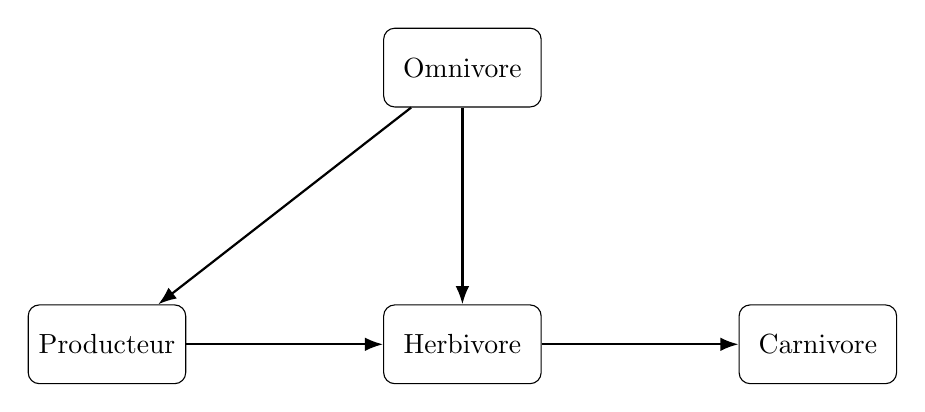
\begin{tikzpicture}[
    node distance=2.5cm and 2.5cm,
    every node/.style={draw, rounded corners, align=center, minimum width=2cm, minimum height=1cm},
    arrow/.style={-{Latex}, thick},
    ]

% Noeuds
\node (producteur) {Producteur};
\node[right=of producteur] (herbivore) {Herbivore};
\node[right=of herbivore] (carnivore) {Carnivore};
\node[above=of herbivore] (omnivore) {Omnivore};

% Flèches principales
\draw[arrow] (producteur) -- (herbivore);
\draw[arrow] (herbivore) -- (carnivore);

% Flèches de l'omnivore
\draw[arrow] (omnivore) -- (herbivore);
\draw[arrow] (omnivore) -- (producteur);

\end{tikzpicture}

\end{document}
